% Created 2012-02-24 Fri 12:26
\documentclass[a4paper]{article}
\usepackage[utf8]{inputenc}
\usepackage[T1]{fontenc}
\usepackage{fixltx2e}
\usepackage{graphicx}
\usepackage{longtable}
\usepackage{float}
\usepackage{wrapfig}
\usepackage{soul}
\usepackage{textcomp}
%\usepackage{marvosym}
%\usepackage{wasysym}
\usepackage{latexsym}
\usepackage{amssymb}
\usepackage{hyperref}
\tolerance=1000
\usepackage{verbatim}
\providecommand{\alert}[1]{\textbf{#1}}

\title{AWAP GRIDS overview}
\author{Ivan Hanigan}
\date{\today}
\hypersetup{
  pdfkeywords={},
  pdfsubject={},
  pdfcreator={Emacs Org-mode version 7.8.03}}

\begin{document}

\maketitle

\setcounter{tocdepth}{3}
\tableofcontents
\vspace*{1cm}
\hrule

\section{Introduction}
\label{sec-1}

NCEPH holds Australian Bureau of Meteorology data for all stations from 1990 to 2010 \cite{NationalClimateCentreoftheBureauofMeteorology:2005}.
The aim of this project is to download the Australian Water Availability Project (AWAP) gridded datasets \cite{Jones2009}.  In particular we want the vapour pressure data from 2010 so that we don't have to buy it again.  We want to compare it with the station data to see if they are close.
\subsection{code}
\label{sec-1-1}













I am also testing the use of R in Emacs orgmode \cite{Schulte}.
\section{Tests}
\label{sec-2}



\begin{verbatim}
 helloworld2
\end{verbatim}
=helloworld
\section{Tools}
\label{sec-3}
\subsection{tools}
\label{sec-3-1}
\subsection{vars}
\label{sec-3-2}

\begin{comment}
this is a test
\end{comment}




\begin{center}
\begin{tabular}{lll}
 rainfall     &  totals    &  daily  \\
 temperature  &  maxave    &  daily  \\
 temperature  &  minave    &  daily  \\
 vprp         &  vprph09   &  daily  \\
 vprp         &  vprph15   &  daily  \\
 solar        &  solarave  &  daily  \\
 ndvi         &  ndviave   &  month  \\
\end{tabular}
\end{center}
\subsection{get data range}
\label{sec-3-3}

A function to get the data for a met variable on a day is called for a range of dates
\subsection{read asciigrid2}
\label{sec-3-4}

A function to get the data from a grid to a long table
\subsection{grid2csv}
\label{sec-3-5}
\section{Load}
\label{sec-4}
\subsection{TASKS}
\label{sec-4-1}
\subsubsection{\textbf{TODO} SET UP TO DO YEAR/MONTH}
\label{sec-4-1-1}
\subsection{download}
\label{sec-4-2}
\subsection{uncompress and transform to long csv}
\label{sec-4-3}
\section{CHECK}
\label{sec-5}




The grid for a particular day is shown in \ref{fig:fig1.jpg}
\begin{figure}[!h]
\centering
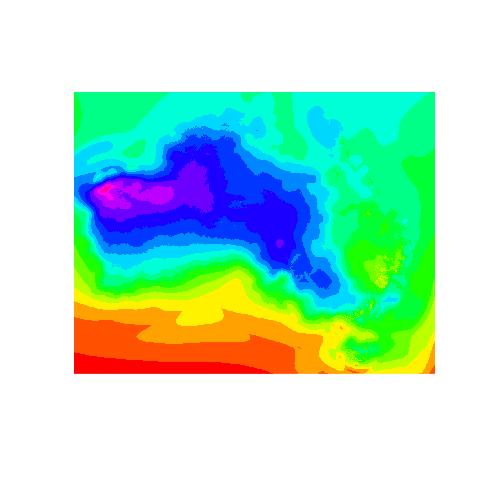
\includegraphics[width=\textwidth]{fig1.jpg}
\caption{fig1.jpg}
\label{fig:fig1.jpg}
\end{figure}
\section{Load csv to delphe}
\label{sec-6}
\subsection{tested Rpostgresql, decide to use COPY instead}
\label{sec-6-1}
\subsection{use COPY instead}
\label{sec-6-2}
\subsubsection{TASKS}
\label{sec-6-2-1}
\begin{itemize}

\item \textbf{TODO} REMOVE newnode add grids?\\
\label{sec-6-2-1-1}%
\end{itemize} % ends low level
\subsubsection{code}
\label{sec-6-2-2}
\subsection{check for duplicates}
\label{sec-6-3}
\subsubsection{TASKS}
\label{sec-6-3-1}
\begin{itemize}

\item \textbf{TODO} insert BoM response about duplicates in January\\
\label{sec-6-3-1-1}%
\item \textbf{TODO} build a test function to check for this at download\\
\label{sec-6-3-1-2}%
\end{itemize} % ends low level
\subsubsection{code}
\label{sec-6-3-2}

This will be code
\subsection{check for missing days}
\label{sec-6-4}
\subsubsection{TASKS}
\label{sec-6-4-1}
\begin{itemize}

\item \textbf{TODO} check4missings\\
\label{sec-6-4-1-1}%
\end{itemize} % ends low level
\subsubsection{code}
\label{sec-6-4-2}

This will be code
\section{check against a station}
\label{sec-7}

Now we can select a timeseries of values for both a pixel and a station and see how well they correspond. 
\subsection{TASKS}
\label{sec-7-1}
\subsubsection{\textbf{TODO} join the station and grid query to one query}
\label{sec-7-1-1}

   \texttt{SCHEDULED:} \textit{2012-02-15 Wed 14:20}
\subsubsection{\textbf{TODO} calcute RMSE and R2 for August only}
\label{sec-7-1-2}
\subsubsection{\textbf{TODO} change the avg(val) to a IDW based on the cell centres}
\label{sec-7-1-3}
\subsection{code}
\label{sec-7-2}




The association of the grid and station data for a particular station is shown in \ref{fig:fig2.jpg}
\begin{figure}[!h]
\centering
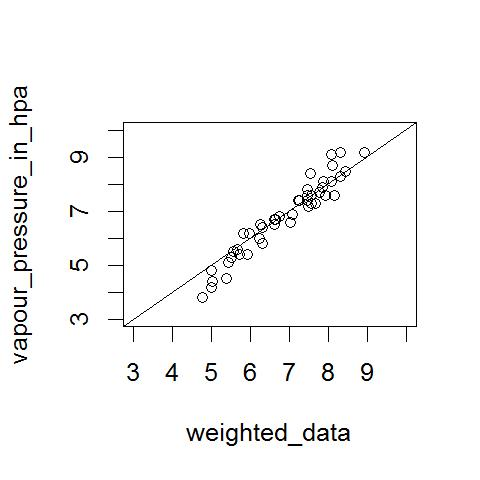
\includegraphics[width=\textwidth]{fig2.jpg}
\caption{fig2.jpg}
\label{fig:fig2.jpg}
\end{figure}
\clearpage
\section{DO}
\label{sec-8}
\subsection{write function to extract timeseries}
\label{sec-8-1}
\subsection{test function}
\label{sec-8-2}
\subsection{publish function}
\label{sec-8-3}
\section{References}
\label{sec-9}

\bibliographystyle{unsrt}
\bibliography{I:/references/library}
\section{Metadata}
\label{sec-10}
\subsection{metadata-init}
\label{sec-10-1}
\subsection{insert study id}
\label{sec-10-2}
\subsection{get list of files already entered}
\label{sec-10-3}


\begin{verbatim}

newnode(dsc='get list of files already entered', clearpage = F, ttype='transformations', nosectionheading = T,
 o = 'get list of files already entered',append = T,end_doc = F,
 notes='',echoCode = FALSE,
 code=NA)

 # newnode first get the list of files I had previously entered
 fileDscr <- dbGetQuery(oracle,sprintf(
 "SELECT * 
 FROM filedscr 
 where IDno = '%s' 
 order by FILETYPE
 ",idno))
 head(fileDscr)
 fileDscr[,1:4]
 write.csv(fileDscr,file.path('metadata','filedscr.csv'),row.names=F) 

# newnode get filedscr
# source(dir('run',pattern = 'metadata_metadata', full.names=T))
\end{verbatim}
\subsection{add a new file}
\label{sec-10-4}


\begin{verbatim}

newnode(dsc='add a new file', clearpage = F, ttype='transformations', nosectionheading = T,
 o = 'add a new file',append = T,end_doc = F,
 notes='',echoCode = FALSE,
 code=NA)

 f <- add_filedscr(fileid = 1, idno = s$IDNO, ask=T)
 f$FILELOCATION <- '-d delphe -s awap_grids'
\end{verbatim}
\subsection{data}
\label{sec-10-5}
\subsubsection{include data desc for file1}
\label{sec-10-5-1}
\subsubsection{include data desc for file2}
\label{sec-10-5-2}
\subsection{analysis}
\label{sec-10-6}
\subsection{document}
\label{sec-10-7}
\subsubsection{add metadata for the files}
\label{sec-10-7-1}
\subsection{metadata}
\label{sec-10-8}
\subsubsection{add metadata for files to oracle}
\label{sec-10-8-1}
\subsubsection{add metadata for data to oracle}
\label{sec-10-8-2}
\subsubsection{oracle2xml-makeTex}
\label{sec-10-8-3}


 
\subsubsection{create catalogue and ddi xmls}
\label{sec-10-8-4}
\begin{itemize}

\item at work\\
\label{sec-10-8-4-1}%
\item at home\\
\label{sec-10-8-4-2}%
\end{itemize} % ends low level
\subsubsection{edit by browser or code}
\label{sec-10-8-5}
\subsubsection{include OTHRSTDYMAT}
\label{sec-10-8-6}
\subsubsection{synchronise local metadata}
\label{sec-10-8-7}


newnode(dsc='synchronise local metadata', clearpage = F, ttype='metadata$_{\mathrm{sync}}$',
 dontshow$_{\mathrm{doc}}$ = T, notes='',echoCode = FALSE,doc$_{\mathrm{code}}$ = F,
 code=''
 
 s <- dbGetQuery(oracle, paste(\"select * from stdydscr where idno = `\",idno,\"'\", sep = `'))
 matrix(s)
 f <- dbGetQuery(oracle, paste(\"select * from filedscr where idno = `\",idno,\"' order by filetype\", sep = `'))
 f[,1:4]

 d <- dbGetQuery(oracle, paste(\"select * from datadscr where fileid in (\",paste(f\$FILEID, collapse = `,'),\")\", sep = `'))
 d

 \# now overwrite the local copies
 dir(`metadata')
 write.csv(s, `metadata/stdydscr.csv', row.names=F)
 write.csv(f, `metadata/filedscr.csv', row.names=F)
 write.csv(d, `metadata/datadscr.csv', row.names=F)


 doclist <- dir(file.path(`I:/My Dropbox/projects/0.3 Catalogue/publishddi',idno), pattern = tolower(idno))
 doclist
 
 for(doc in doclist)\{
 file.copy(file.path(`I:/My Dropbox/projects/0.3 Catalogue/publishddi',idno,doc), file.path(`metadata',doc), overwrite = T)
 \}
 
 doc <- dir(file.path(`I:/My Dropbox/projects/0.3 Catalogue/publishddi',idno,'reports'), pattern = `pdf')
 file.copy(file.path(`I:/My Dropbox/projects/0.3 Catalogue/publishddi',idno,'reports',doc), file.path(`metadata',gsub(`_doc','_metadata',doc)), overwrite = T)
 
 ``)
source(dir(`run',pattern='metadata$_{\mathrm{sync}}$', full.names=T) )
\subsubsection{further edits}
\label{sec-10-8-8}


  \# notes=' `,echoCode = FALSE,doc$_{\mathrm{code}}$ = F,
 \# code=''


 
 \# \# carefully
 \# sqlQuery(oracle, 
 \# paste(\"select * from datadscr 
 \# where LABL = `wedge'
 \# and fileid in (\",paste(f\$FILEID, collapse = `,'),\")
 \# \", sep = `'), as.is = T)
 
 \# sqlQuery(oracle, 
 \# paste(\"update datadscr 
 \# set NOTES = `Wedge represents the search radius in kilometres for hotspots around the focal pollution monitor (25  50  75 100 150 200 300 400 500)'
 \# where LABL = `wedge'
 \# and fileid in (\",paste(f\$FILEID, collapse = `,'),\")
 \# \", sep = `'), as.is = T)

 \# sqlQuery(oracle, 
 \# paste(\"select * from datadscr 
 \# where LABL = `idma'
 \# and fileid in (\",paste(f\$FILEID, collapse = `,'),\")
 \# \", sep = `'), as.is = T)
 
 \# sqlQuery(oracle, 
 \# paste(\"update datadscr 
 \# set NOTES = ` IDMA (InDex MacArthur) should be more properly called FFDI (Forest Fire Danger Index), and represents the calculated FFDI at the location of the pollution station on that day.'
 \# where LABL = `idma'
 \# and fileid in (\",paste(f\$FILEID, collapse = `,'),\")
 \# \", sep = `'), as.is = T)

 
 \# ``)
  
\subsection{archive}
\label{sec-10-9}
\subsubsection{manage access}
\label{sec-10-9-1}


 \# notes='',echoCode = FALSE,doc$_{\mathrm{code}}$ = F,
 \# code=''


 
 \# dbSendUpdate(ch,
 \# `grant select on all tables in schema bio$_{\mathrm{events}}$ to bio'
 \# )

 
 \# ``)
 
\subsubsection{migrate data to final location}
\label{sec-10-9-2}


newnode(dsc='migrate data to final location',ttype='archive',
 dontshow$_{\mathrm{doc}}$ = T, notes='',echoCode = FALSE,doc$_{\mathrm{code}}$ = F, clearpage = F,
 code=''
 
 ``)
 
\subsubsection{archive milestone dataset}
\label{sec-10-9-3}


newnode(dsc='archive milestone dataset',ttype='archive',
 dontshow$_{\mathrm{doc}}$ = T, notes='',echoCode = FALSE,doc$_{\mathrm{code}}$ = F, clearpage = F,
 code=''
 
 \# use synchronise it to send from dbxwd to wd (minus metadata) ie ``I:/projects/1.302 Biomass/analysis/exposures/event validation'' 
 \# only a selection of the files
 
 \# Mount truecrypt volume to K
 dir(`K:')
 outdir <- `K:/projects/1.302 Biomass/analysis/exposures/event validation'
 dir.create(outdir, recursive=T)
 \# \# newnode migrate CURRENT$_{\mathrm{FireEvents}}$.mdb
 t(fileDscr[which(fileDscr\$FILENAME == 'CURRENT_FireEvents.mdb'),])
 outfile <- fileDscr[which(fileDscr$FILENAME == `CURRENT$_{\mathrm{FireEvents}}$.mdb'),]
 file.copy(file.path(outfile\$FILELOCATION,outfile\$FILENAME), file.path(outdir,outfile\$FILENAME))
 file.copy(file.path(outfile\$FILELOCATION,'Mousehook.dll'), file.path(outdir,'Mousehook.dll'))
 \# I could just use the GUI?
 ``)
 
\subsection{the end}
\label{sec-10-10}


newnode(dsc = `The end', clearpage = F, ttype = `report', nosectionheading = T,
dontshow = T,
append = T,
document='sweave',
end$_{\mathrm{doc}}$ = T)


 oldwd <- getwd()
 setwd(`reports')
 Sweave(`bio$_{\mathrm{validated}}$$_{\mathrm{bushfire}}$$_{\mathrm{events}}$$_{\mathrm{transformations}}$$_{\mathrm{doc}}$.Rnw')

 setwd(oldwd)
\section{Archives}
\label{sec-11}
\subsection{TASKS}
\label{sec-11-1}
\subsubsection{\textbf{TODO} add to nceph unrestricted and github}
\label{sec-11-1-1}
\subsection{code}
\label{sec-11-2}

This is the achiving node.
\section{End}
\label{sec-12}



\begin{comment}
source('~/my dropbox/tools/transformations.r')
source('run/transformations.r')
"i:\My Dropbox\tools\transformationscolour.py"  AWAP_GRIDS_transformations.txt   AWAP_GRIDS_transformations
\end{comment}

\end{document}
